% ============================================================================
% CHƯƠNG 3: THIẾT KẾ HỆ THỐNG
% ============================================================================
\chapter{THIẾT KẾ HỆ THỐNG}

Chương này mô tả thiết kế chi tiết của hệ thống L-RAG (LegalDiff), bao gồm kiến trúc tổng thể 3-Phase, thiết kế data models, và chi tiết từng module trong pipeline xử lý.

% ============================================================================
\section{Kiến trúc Tổng thể 3-Phase}
% ============================================================================

Hệ thống L-RAG được thiết kế theo kiến trúc pipeline tuần tự gồm 3 Phase, với 11 module được phân bổ như sau:

\begin{figure}[H]
    \centering
    \begin{tikzpicture}[node distance=1.8cm, auto]
        \tikzstyle{phase} = [rectangle, draw, fill=blue!5, text width=6.5cm, text centered, minimum height=2.2cm, rounded corners]
        \tikzstyle{data} = [rectangle, draw, fill=green!5, text width=4.5cm, text centered, minimum height=0.9cm, rounded corners]
        \tikzstyle{arrow} = [thick,->,>=stealth]

        \node [data] (v1) {V1: PDF/DOCX};
        \node [data, right=5cm of v1] (v2) {V2: PDF/DOCX};

        \node [phase, below=0.8cm of $(v1)!0.5!(v2)$] (p1) {\textbf{PHASE 1 — Ingestion}\\Module 1: Docling Parser | Module 2: LSU Chunker | Module 3: HybridGraphBuilder};
        \node [data, below=of p1] (d1) {Legal DOM Tree + LSU Chunks + Knowledge Graph};
        \node [phase, below=of d1] (p2) {\textbf{PHASE 2 — Alignment}\\Module 4: BGE-M3 | Module 5: Similarity Matrix | Module 6: Hungarian Matcher | Module 7: Qdrant};
        \node [data, below=of p2] (d2) {DiffPairCatalog: matched / added / deleted / split / merged};
        \node [phase, below=of d2] (p3) {\textbf{PHASE 3 — Comparison}\\Module 8: ACU Prompter | Module 9: LLM Client | Module 10: Verification | Module 11: Report};
        \node [data, below=of p3] (d3) {Comparison Report (JSON + Markdown)};

        \draw [arrow] (v1) |- (p1);
        \draw [arrow] (v2) |- (p1);
        \draw [arrow] (p1) -- (d1);
        \draw [arrow] (d1) -- (p2);
        \draw [arrow] (p2) -- (d2);
        \draw [arrow] (d2) -- (p3);
        \draw [arrow] (p3) -- (d3);
    \end{tikzpicture}
    \caption{Kiến trúc tổng thể 3-Phase của hệ thống L-RAG}
    \label{fig:architecture_overview}
\end{figure}

\subsection{Phase 1 — Ingestion \& Knowledge Representation}

Chịu trách nhiệm chuyển đổi file PDF/DOCX đầu vào thành cấu trúc dữ liệu có tổ chức, bao gồm: cây Legal DOM, danh sách LSU chunk, và Hybrid Knowledge Graph (Kuzu + ChromaDB). Phase 1 hoàn toàn deterministic, không sử dụng \gls{llm}.

\subsection{Phase 2 — Indexing \& Alignment}

Thực hiện ghép cặp tối ưu các article/clause giữa hai phiên bản bằng BGE-M3 embedding, ma trận tương đồng đa trọng số, và thuật toán Hungarian. Đầu ra là DiffPairCatalog chứa danh sách các cặp article đã được match, cùng các article được thêm mới (added), xóa bỏ (deleted), tách (split), và gộp (merged).

\subsection{Phase 3 — Generative Comparison}

Giai đoạn duy nhất sử dụng \gls{llm}. Mỗi cặp article đã match được đưa qua pipeline: (1) LLM trích xuất Atomic Comparison Unit (\gls{acu}), (2) xác minh evidence 3 tầng, (3) tổng hợp báo cáo. LLM hoạt động ở nhiệt độ cực thấp ($T=0.05$) và bị ràng buộc chặt chẽ bởi prompt để đảm bảo Zero Hallucination.

% ============================================================================
\section{Thiết kế Data Models}
% ============================================================================

\subsection{Legal DOM Tree}

Cấu trúc cây pháp lý mô hình hóa đầy đủ hệ thống phân cấp của văn bản pháp lý Việt Nam. Mỗi node trong cây là một Pydantic BaseModel với định danh duy nhất (node\_id) được sinh tự động qua UUID.

\begin{figure}[H]
    \centering
    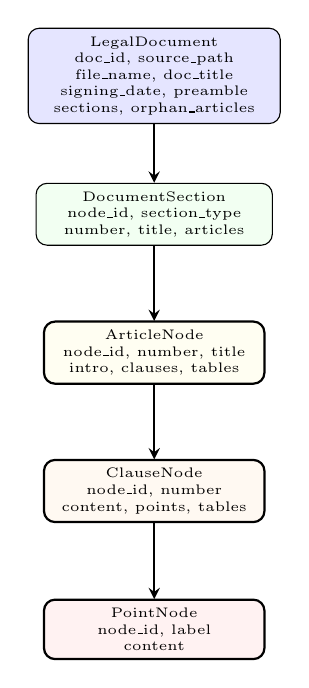
\begin{tikzpicture}[sibling distance=14em, level distance=5em,
        every node/.style={draw, rectangle, rounded corners, align=center, minimum width=2.8cm, font=\tiny, inner sep=3pt},
        edge from parent/.style={draw, -{stealth}, thick}]
        \node [fill=blue!10, minimum width=3.2cm] {LegalDocument\\doc\_id, source\_path\\file\_name, doc\_title\\signing\_date, preamble\\sections, orphan\_articles}
            child { node [fill=green!5, minimum width=3cm] {DocumentSection\\node\_id, section\_type\\number, title, articles}
                child { node [fill=yellow!5] {ArticleNode\\node\_id, number, title\\intro, clauses, tables}
                    child { node [fill=orange!5] {ClauseNode\\node\_id, number\\content, points, tables}
                        child { node [fill=red!5] {PointNode\\node\_id, label\\content}
                        }
                    }
                }
            };
    \end{tikzpicture}
    \caption{Cấu trúc Legal DOM Tree đầy đủ với các trường dữ liệu chính}
    \label{fig:legal_dom}
\end{figure}

\subsection{LSU Chunk}

Mỗi LSU chunk là đơn vị được embedding, với breadcrumb prefix cung cấp ngữ cảnh về vị trí trong cây pháp lý. Bảng~\ref{tab:lsu_chunk_schema} mô tả các trường dữ liệu:

\begin{table}[H]
    \centering
    \caption{Lược đồ dữ liệu LSU Chunk}
    \label{tab:lsu_chunk_schema}
    \begin{tabularx}{\textwidth}{l l X}
        \toprule
        \textbf{Trường} & \textbf{Kiểu} & \textbf{Mô tả}\\
        \midrule
        chunk\_id & str & Định danh duy nhất (UUID)\\
        doc\_id & str & Liên kết đến LegalDocument\\
        source\_node\_id & str & Liên kết đến ArticleNode hoặc ClauseNode\\
        breadcrumb & str & Ví dụ: ``[Chương II > Điều 5 > Khoản 3]''\\
        content\_with\_prefix & str & breadcrumb + ``\textbackslash n'' + raw\_content — được embedding\\
        raw\_content & str & Nội dung thuần, không có breadcrumb\\
        content\_type & ContentType & TEXT, TABLE, hoặc MIXED\\
        tables\_json & list[dict] & Bảng biểu dạng JSON có cấu trúc\\
        char\_count & int & Số ký tự của raw\_content (tự động tính)\\
        \bottomrule
    \end{tabularx}
\end{table}

\subsection{DiffPair và DiffPairCatalog}

\textbf{DiffPair} biểu diễn một cặp article được alignment, hỗ trợ 5 loại match\_type: MATCHED, ADDED, DELETED, SPLIT, MERGED. Mỗi DiffPair chứa confidence\_score tổng hợp và các score thành phần (semantic, jaro\_winkler, ordinal\_proximity).

\textbf{DiffPairCatalog} là container chứa toàn bộ kết quả alignment, với các thuộc tính computed: matched\_pairs, added\_nodes, deleted\_nodes, split\_cases, merged\_cases, và phương thức summary() trả về thống kê số lượng.

\subsection{ACU Output và Comparison Report}

\textbf{ACUOutput} (\gls{acu} — Atomic Comparison Unit) là đơn vị thay đổi nguyên tử — mỗi ACU mô tả đúng một thay đổi. Các trường chính:

\begin{itemize}
    \item \texttt{change\_type}: 1 trong 6 loại — numerical, terminology, structural, addition, deletion, reorder
    \item \texttt{original\_value} / \texttt{new\_value}: Giá trị trước và sau thay đổi
    \item \texttt{verbatim\_evidence\_v1} / \texttt{verbatim\_evidence\_v2}: Trích dẫn nguyên văn từ source — nền tảng của Zero-Hallucination
    \item \texttt{confidence}: Độ tin cậy của LLM [0.0, 1.0]
\end{itemize}

\textbf{ComparisonReport} tổng hợp kết quả cuối cùng: danh sách ACU đã xác minh (passed), ACU bị loại (rejected) kèm lý do, executive summary bằng tiếng Việt, và báo cáo Markdown đầy đủ.

% ============================================================================
\section{Phase 1 — Ingestion \& Knowledge Representation}
% ============================================================================

\subsection{Module 1 — LegalDocumentParser}

Parser sử dụng Docling \cite{docling2024} làm engine chính, với Marker/Surya \cite{marker2024,surya2024} làm fallback \gls{ocr} cho PDF scan. Luồng xử lý:

\begin{enumerate}[label=(\arabic*)]
    \item Xác thực file đầu vào (phải là .pdf, .docx, hoặc .doc)
    \item Parse bằng Docling: sử dụng \texttt{DocumentConverter} với cấu hình \texttt{PdfPipelineOptions(do\_ocr=False, do\_table\_structure=True)}
    \item Tính toán chất lượng parse: trung bình confidence của các text item và tỷ lệ trang có confidence thấp ($< 0.5$)
    \item Nếu confidence thấp ($< 0.75$) hoặc tỷ lệ trang thấp $> 0.30$: kích hoạt OCR fallback
    \item Export Docling output sang Markdown, trích xuất bảng dạng \texttt{TableData} (có row\_span/col\_span)
    \item Xây dựng Legal DOM tree bằng state machine duyệt từng dòng
\end{enumerate}

State machine DOM builder hoạt động với độ phức tạp $O(n)$ với $n$ là số dòng văn bản. Tại mỗi dòng, regex matching được thực hiện theo thứ tự ưu tiên: Section > Article > Clause > Point. Khi gặp node mới ở cấp cao hơn, toàn bộ node cấp thấp hơn được flush (đẩy vào cây).

\subsection{Module 2 — LSU Chunker}

Chunker chuyển đổi LegalDocument thành danh sách LSU chunk theo hai mức:

\begin{enumerate}[label=(\arabic*)]
    \item \textbf{Article-level chunk}: Nội dung = article.intro + preview của các clause (150 ký tự/clause). Breadcrumb = ``[Section > Article N. Title]''.
    \item \textbf{Clause-level chunk}: Nội dung = clause.content + toàn bộ point sub-contents. Breadcrumb = ``[Section > Article N > Clause M]''.
\end{enumerate}

Với clause có nội dung vượt quá \texttt{max\_chunk\_chars} (mặc định 2000), \texttt{\_SentenceSplitter} được kích hoạt:

\begin{lstlisting}[language=Python, caption={Thuật toán SentenceSplitter — chia clause dài tại ranh giới câu}, label={lst:sentence_splitter}]
class _SentenceSplitter:
    def split(self, text: str) -> list[str]:
        if len(text) <= self.max_chars:
            return [text]

        sentences = _RE_SENTENCE_BOUNDARY.split(text)
        if len(sentences) == 1:
            return self._hard_split(text)  # fallback

        chunks = []
        current = ""
        for sent in sentences:
            if len(current) + len(sent) > self.max_chars and current:
                chunks.append(current.strip())
                # Overlap: last overlap_chars of previous chunk
                current = current[-self.overlap_chars:] + sent
            else:
                current += sent
        if current.strip():
            chunks.append(current.strip())
        return chunks
\end{lstlisting}

\subsection{Module 3 — HybridGraphBuilder}

Xây dựng Hybrid Knowledge Graph kết hợp hai cơ sở dữ liệu:

\begin{itemize}
    \item \textbf{Kuzu Embedded Graph DB} \cite{kuzu2024}: Lưu trữ cấu trúc đồ thị với 2 node table (Document, LegalNode) và 3 edge table (CONTAINS, PRECEDES, REFERENCES). Liên kết REFERENCES được phát hiện tự động qua regex phát hiện cụm ``theo quy định tại Điều X'' trong nội dung văn bản.
    \item \textbf{ChromaDB Vector DB} \cite{chromadb2024}: Lưu trữ vector embedding của các LSU chunk, liên kết với graph qua trường \texttt{node\_id} trong metadata.
\end{itemize}

Cả hai DB được liên kết với nhau qua \texttt{node\_id} — mỗi LSU chunk trong ChromaDB có metadata chứa node\_id trỏ đến node tương ứng trong Kuzu. Điều này cho phép truy vấn hybrid: tìm kiếm ngữ nghĩa trong ChromaDB, sau đó traversals đồ thị trong Kuzu để lấy ngữ cảnh.

\begin{figure}[H]
    \centering
    \begin{tikzpicture}[node distance=2cm, auto]
        \tikzstyle{db} = [rectangle, draw, fill=blue!5, text width=3.5cm, text centered, minimum height=2cm, rounded corners]
        \tikzstyle{arrow} = [thick,<->,>=stealth]

        \node [db] (kuzu) {\textbf{Kuzu Graph DB}\\Document Node\\LegalNode (Article/Clause)\\CONTAINS, PRECEDES,\\REFERENCES edges};
        \node [db, right=4cm of kuzu] (chroma) {\textbf{ChromaDB Vector DB}\\LSU Chunk embeddings\\VectorMetadata\\node\_id (link)};

        \draw [arrow] (kuzu) -- node [above] {\texttt{node\_id}} (chroma);
    \end{tikzpicture}
    \caption{Hybrid Knowledge Graph: Kuzu (graph structure) và ChromaDB (semantic vectors) liên kết qua node\_id}
    \label{fig:hybrid_graph}
\end{figure}

% ============================================================================
\section{Phase 2 — Indexing \& Alignment}
% ============================================================================

\subsection{Module 4 — BGEM3Manager}

Quản lý mô hình BGE-M3 \cite{chen2024bge} cho embedding. Mô hình được tải ở chế độ \gls{fp16} qua thư viện FlagEmbedding:

\begin{lstlisting}[language=Python, caption={Khởi tạo BGE-M3 Manager với dual embedding}, label={lst:bge_m3}]
class BGEM3Manager:
    def __init__(self, model_name="BAAI/bge-m3", use_fp16=True,
                 batch_size=16, max_length=1024):
        self._model = BGEM3FlagModel(
            model_name_or_path=model_name,
            use_fp16=use_fp16,
            device=device
        )
\end{lstlisting}

Phương thức chính \texttt{embed\_article\_nodes()} và \texttt{embed\_clause\_nodes()} tạo hai vector cho mỗi node:

\begin{itemize}
    \item \textbf{Structural embedding}: Đầu vào = ``Điều \{ordinal\}: \{title\}'' (article) hoặc ``Điều \{parent\} Khoản \{n\}: \{preview[:80]\}'' (clause). \texttt{max\_length=512}.
    \item \textbf{Semantic embedding}: Đầu vào = ``[breadcrumb]\textbackslash n\{full\_text\}''. \texttt{max\_length=1024}.
\end{itemize}

Mỗi node embedding được đóng gói trong \texttt{NodeEmbeddings} với đầy đủ dense vectors, sparse vectors, và payload cho Qdrant.

\subsection{Module 5 — Similarity Matrix}

Ma trận tương đồng $S \in \mathbb{R}^{N \times M}$ được tính từ ba ma trận thành phần:

\begin{equation}
    S = \alpha \cdot S_{\text{cos}} + \beta \cdot S_{\text{jw}} + \gamma \cdot S_{\text{ord}}
    \label{eq:sim_matrix_impl}
\end{equation}

\begin{lstlisting}[language=Python, caption={Xây dựng ma trận tương đồng đa trọng số}, label={lst:sim_matrix}]
def compute_similarity_matrix(v1_records, v2_records, config):
    N, M = len(v1_records), len(v2_records)

    # 1. Semantic cosine similarity (alpha=0.6)
    v1_mat = np.stack([r.semantic_vec for r in v1_records])
    v2_mat = np.stack([r.semantic_vec for r in v2_records])
    v1_mat = _l2_normalize(v1_mat)
    v2_mat = _l2_normalize(v2_mat)
    S_cos = v1_mat @ v2_mat.T

    # 2. Jaro-Winkler title similarity (beta=0.3)
    S_jw = jaro_winkler_matrix(v1_records, v2_records)

    # 3. Ordinal proximity (gamma=0.1)
    S_ord = ordinal_proximity_matrix(v1_records, v2_records, N, M)

    # Weighted combination
    S = (config.w_semantic * S_cos +
         config.w_jaro_winkler * S_jw +
         config.w_ordinal * S_ord)
    return np.clip(S, 0.0, 1.0)
\end{lstlisting}

Độ phức tạp: $O(N \cdot M \cdot d)$ cho cosine similarity (với $d=1024$), $O(N \cdot M)$ cho Jaro-Winkler và ordinal proximity.

\subsection{Module 6 — Hungarian Matcher \& Split/Merge Detection}

Thuật toán Hungarian được áp dụng trên ma trận chi phí $C = 1 - S$:

\begin{lstlisting}[language=Python, caption={Hungarian matching với split/merge detection}, label={lst:hungarian}]
def hungarian_match(similarity_matrix, match_threshold=0.65):
    cost = 1.0 - similarity_matrix
    row_ind, col_ind = linear_sum_assignment(cost)

    matched_pairs = []
    for i, j in zip(row_ind, col_ind):
        score = 1.0 - cost[i][j]
        if score >= match_threshold:
            matched_pairs.append((i, j, score))

    v1_unmatched = [i for i in range(N) if i not in row_ind[matched]]
    v2_unmatched = [j for j in range(M) if j not in col_ind[matched]]
    return matched_pairs, v1_unmatched, v2_unmatched
\end{lstlisting}

Sau khi Hungarian matching, các node unmatched được đưa qua \texttt{detect\_split\_merge()}:

\begin{itemize}
    \item \textbf{Merge detection}: Với mỗi cặp V1\_$i$, V1\_$j$ (unmatched) và V2\_$k$ (unmatched), kiểm tra $\cos(\text{embed}(T_i^{V1} \parallel T_j^{V1}), \text{embed}(T_k^{V2})) \geq 0.80$.
    \item \textbf{Split detection}: Ngược lại — một V1 unmatched với hai V2 unmatched.
\end{itemize}

Độ phức tạp của split/merge detection: $O(U_1^2 \cdot U_2 + U_1 \cdot U_2^2)$ với $U_1, U_2$ là số lượng node unmatched. Với văn bản pháp lý thông thường ($U < 10$), chi phí này không đáng kể.

\subsection{Module 7 — Qdrant Indexer}

Qdrant \cite{qdrant2024} được sử dụng làm vector database cho Phase 2, hỗ trợ multi-vector storage:

\begin{itemize}
    \item Mỗi điểm (point) trong Qdrant chứa 2 named dense vector (``structural'' và ``semantic'', 1024 chiều) và 2 named sparse vector (``structural\_sparse'' và ``semantic\_sparse'').
    \item Sử dụng HNSW index \cite{hnsw} với $M=16$, $\text{ef\_construct}=200$, cosine distance.
    \item Payload index trên 6 trường: version, node\_type, doc\_id, node\_id, ordinal, article\_number — cho phép lọc nhanh theo version (V1/V2).
\end{itemize}

Việc chuyển đổi sparse vector từ BGE-M3 (dạng \texttt{\{token\_string: weight\}}) sang Qdrant-compatible format (dạng \texttt{\{int\_index: weight\}}) thực hiện qua băm token với bucket size $2^{20}$.

% ============================================================================
\section{Phase 3 — Generative Comparison}
% ============================================================================

\subsection{Module 8 — ACU Prompter}

ACU Prompter xây dựng prompt cho LLM với thiết kế \textbf{``transcription, not generation''}. System prompt chứa 6 quy tắc bắt buộc (RULE 1--6), yêu cầu JSON mode, và định nghĩa schema đầu ra chính xác.

User prompt được xây dựng từ template:

\begin{lstlisting}[language=Python, caption={Xây dựng ACU user prompt với context và guidance}, label={lst:acu_prompt}]
def build_acu_user_prompt(raw_text_v1, raw_text_v2,
                          breadcrumb_v1="", breadcrumb_v2="",
                          match_type="matched") -> str:
    context = f"Vi tri V1: {breadcrumb_v1}\nVi tri V2: {breadcrumb_v2}"

    guidance = {
        "matched": "Tim nhung thay doi tinh vi ve noi dung.",
        "added": "V2 moi hoan toan. Tao 1 ACU addition.",
        "deleted": "V1 da bi xoa. Tao 1 ACU deletion.",
        "split": "V1 bi TACH. Xac dinh phan giu nguyen vs thay doi.",
        "merged": "Nhieu V1 duoc GOP. Xac dinh phan giu nguyen vs xoa.",
    }[match_type]

    return f"""{context}

    HUONG DAN: {guidance}

    <v1_text>{raw_text_v1}</v1_text>
    <v2_text>{raw_text_v2}</v2_text>

    Tra ve CHI MOT JSON object voi danh sach acus."""
\end{lstlisting}

Việc bọc văn bản trong XML tags \texttt{<v1\_text>} và \texttt{<v2\_text>} giúp LLM phân biệt rõ ràng ranh giới giữa hai phiên bản, giảm thiểu nhầm lẫn.

\subsection{Module 9 — Local LLM Client}

LLM Client giao tiếp với llama.cpp server \cite{llamacpp2024} qua OpenAI-compatible API tại \texttt{http://localhost:8000/v1}, sử dụng thư viện \texttt{openai.AsyncOpenAI}.

\begin{table}[H]
    \centering
    \caption{Cấu hình LLM Client cho từng tác vụ}
    \label{tab:llm_config}
    \begin{tabularx}{\textwidth}{X c c c X}
        \toprule
        \textbf{Tác vụ} & \textbf{T} & \textbf{Max Tokens} & \textbf{JSON Mode} & \textbf{Mục đích}\\
        \midrule
        ACU Extraction & 0.05 & 4096 & Bắt buộc & Trích xuất thay đổi gần deterministic\\
        Executive Summary & 0.3 & 1024 & Bắt buộc & Tổng hợp báo cáo (có kiểm soát)\\
        \bottomrule
    \end{tabularx}
\end{table}

Hai LLM client riêng biệt được khởi tạo với temperature khác nhau, tránh cross-contamination giữa tác vụ extraction (cần độ chính xác cao) và summarization (cần văn phong tự nhiên).

Cơ chế retry với exponential backoff: \texttt{delay = 1.0 * 2\textasciicircum attempt}, tối đa 3 lần retry cho các lỗi kết nối và timeout. Model mặc định: Qwen2.5-7B-Instruct \cite{qwen2025}, chạy qua llama.cpp với lượng tử hóa Q4\_K\_M (GGUF), tiêu thụ $\sim$5GB \gls{vram}.

\subsection{Module 10 — Verification Engine (3 Tầng)}

Verification Engine là trái tim của cơ chế Zero-Hallucination, hoạt động qua 3 tầng với cấu hình:

\begin{table}[H]
    \centering
    \caption{Cấu hình Verification Engine}
    \label{tab:verification_config}
    \begin{tabularx}{\textwidth}{X c X}
        \toprule
        \textbf{Tham số} & \textbf{Giá trị} & \textbf{Mô tả}\\
        \midrule
        fuzzy\_match\_threshold & 0.85 & Ngưỡng SequenceMatcher ratio cho fuzzy match\\
        min\_evidence\_length & 5 & Evidence < 5 ký tự bị skip (tránh false positive)\\
        normalize\_whitespace & True & Chuẩn hóa khoảng trắng trước khi so sánh\\
        strict\_numerical & True & Yêu cầu 100\% số liệu khớp với source\\
        numerical\_context\_window & 50 & Cửa sổ ngữ cảnh khi định vị số trong văn bản\\
        min\_confidence\_to\_include & 0.4 & ACU có confidence < 0.4 bị pre-filter\\
        \bottomrule
    \end{tabularx}
\end{table}

\subsubsection{Tầng 1 — Evidence Verification}

Quy trình 3 bước cascading cho mỗi evidence string:

\begin{enumerate}[label=(\arabic*)]
    \item \textbf{Exact substring match}: \texttt{evidence in raw\_text} — nhanh nhất, chính xác nhất
    \item \textbf{Normalized match}: Chuẩn hóa whitespace, kiểm tra lại — xử lý artifact từ PDF/OCR
    \item \textbf{Fuzzy sliding-window}: \texttt{SequenceMatcher} quét window trên raw\_text (80\%–150\% độ dài evidence). Khớp nếu ratio $\geq 0.85$
\end{enumerate}

Evidence ngắn hơn 5 ký tự được skip (passed) để tránh false positive. ACU với change\_type=ADDITION chỉ kiểm tra evidence V2; DELETION chỉ kiểm tra evidence V1.

\subsubsection{Tầng 2 — Numerical Verification}

Áp dụng riêng cho ACU có change\_type=NUMERICAL. Hệ thống sử dụng 8 regex pattern để trích xuất số từ cả original\_value, new\_value, và raw\_text tương ứng. Các pattern được thiết kế cho định dạng số trong văn bản pháp lý tiếng Việt:

\begin{itemize}
    \item Ngày tháng: \texttt{DD/MM/YYYY}, \texttt{DD-MM-YYYY}, \texttt{D/M/YY}
    \item Phần trăm: \texttt{XX\%}, \texttt{XX,X\%}
    \item Tiền tệ VN: \texttt{XXX.XXX dong}, \texttt{XXX.XXX VND}
    \item Số thập phân, số nguyên
\end{itemize}

Yêu cầu \textbf{strict mode}: 100\% số liệu từ original\_value phải xuất hiện trong V1\_raw\_text, và 100\% số liệu từ new\_value phải xuất hiện trong V2\_raw\_text. Chỉ cần một số không khớp, toàn bộ ACU bị loại.

\subsubsection{Pre-filter}

Trước khi vào verification, ACU có confidence < 0.4 bị loại trực tiếp — đây là các ACU mà chính LLM cũng không chắc chắn, thường là noise.

\subsection{Module 11 — Report Generator}

Pipeline \texttt{GenerativeComparisonPipeline} điều phối toàn bộ Phase 3 qua phương thức \texttt{run\_single()}:

\begin{enumerate}[label=(\arabic*)]
    \item Gọi LLM (T=0.05) trích xuất ACU từ cặp article
    \item Pre-filter: loại ACU confidence < 0.4
    \item Verification: chạy 2 tầng xác minh, phân loại passed/rejected
    \item Gọi LLM (T=0.3) sinh Executive Summary từ danh sách ACU đã passed
    \item Render Markdown report với thống kê, danh sách ACU theo change\_type, và hallucination log
\end{enumerate}

Pipeline hỗ trợ xử lý song song với \texttt{asyncio.Semaphore} (mặc định max\_concurrency=4), cho phép xử lý đồng thời 4 cặp article. Khi LLM summary thất bại, một fallback summary được sinh tự động từ thống kê ACU (không cần LLM).

Báo cáo Markdown đầu ra bao gồm: thông tin chung (report\_id, doc\_id, location), bảng thống kê (total/passed/rejected/hallucination\_rate), Executive Summary, danh sách ACU chi tiết phân nhóm theo change\_type với bằng chứng trích dẫn, và hallucination log.

% ============================================================================
\section{Cấu hình Hệ thống}
% ============================================================================

Toàn bộ tham số vận hành được tập trung trong hai file YAML:

\begin{table}[H]
    \centering
    \caption{Các tham số cấu hình chính của hệ thống}
    \label{tab:config_main}
    \begin{tabularx}{\textwidth}{X c c X}
        \toprule
        \textbf{Tham số} & \textbf{Giá trị} & \textbf{Phase} & \textbf{Vai trò}\\
        \midrule
        max\_chunk\_chars & 2000 & Phase 1 & Kích thước tối đa 1 LSU chunk\\
        overlap\_chars & 200 & Phase 1 & Overlap khi split clause dài\\
        confidence\_threshold & 0.75 & Phase 1 & Ngưỡng kích hoạt OCR fallback\\
        w\_semantic ($\alpha$) & 0.6 & Phase 2 & Trọng số cosine similarity\\
        w\_jaro\_winkler ($\beta$) & 0.3 & Phase 2 & Trọng số Jaro-Winkler\\
        w\_ordinal ($\gamma$) & 0.1 & Phase 2 & Trọng số ordinal proximity\\
        match\_threshold & 0.65 & Phase 2 & Ngưỡng matched pair\\
        split\_merge\_threshold & 0.80 & Phase 2 & Ngưỡng split/merge detection\\
        fuzzy\_match\_threshold & 0.85 & Phase 3 & Ngưỡng fuzzy evidence match\\
        min\_confidence\_to\_include & 0.4 & Phase 3 & Pre-filter confidence\\
        acu\_temperature & 0.05 & Phase 3 & Nhiệt độ LLM cho ACU\\
        summary\_temperature & 0.3 & Phase 3 & Nhiệt độ LLM cho summary\\
        max\_concurrency & 4 & Phase 3 & Số cặp article xử lý song song\\
        \bottomrule
    \end{tabularx}
\end{table}

% ============================================================================
\section{Tech Stack}
% ============================================================================

Bảng~\ref{tab:tech_stack_full} tổng hợp toàn bộ công nghệ sử dụng trong hệ thống:

\begin{table}[H]
    \centering
    \caption{Tech Stack đầy đủ của L-RAG}
    \label{tab:tech_stack_full}
    \begin{tabularx}{\textwidth}{X c X X}
        \toprule
        \textbf{Thành phần} & \textbf{Công nghệ} & \textbf{VRAM} & \textbf{Vai trò}\\
        \midrule
        Document Parser & Docling (IBM) & — & Parse PDF/DOCX, giữ cấu trúc bảng\\
        OCR Fallback & Marker + Surya & — & Xử lý PDF scan chất lượng thấp\\
        Embedding Model & BGE-M3 (FP16) & $\sim$2GB & Dual embedding (structural + semantic)\\
        Graph DB & Kuzu Embedded & — & Lưu trữ cấu trúc đồ thị, REFERENCES edges\\
        Vector DB (Phase 1) & ChromaDB & — & Persistent vector storage cho LSU chunks\\
        Vector DB (Phase 2) & Qdrant & — & Multi-vector storage (dense + sparse)\\
        LLM Server & llama.cpp & — & OpenAI-compatible API server\\
        LLM Model & Qwen2.5-7B (Q4\_K\_M) & $\sim$5GB & ACU extraction + Executive summary\\
        Hungarian Solver & SciPy & — & \texttt{linear\_sum\_assignment}\\
        String Matching & jellyfish + difflib & — & Jaro-Winkler + SequenceMatcher\\
        Data Validation & Pydantic v2 & — & Type-safe data models + validators\\
        API Layer & FastAPI & — & RESTful API cho người dùng cuối\\
        \midrule
        \textbf{Tổng VRAM} & & \textbf{$\sim$7--8GB} & Thoải mái trên RTX 4090 (24GB)\\
        \bottomrule
    \end{tabularx}
\end{table}

\section{Tổng kết Chương}

Chương này đã trình bày thiết kế chi tiết của toàn bộ hệ thống L-RAG qua ba Phase và 11 module:

\begin{enumerate}[label=(\arabic*)]
    \item \textbf{Phase 1 — Ingestion}: Chuyển đổi PDF/DOCX thành Legal DOM Tree và LSU chunks, lưu trữ trong Hybrid Knowledge Graph (Kuzu + ChromaDB) liên kết qua node\_id.
    \item \textbf{Phase 2 — Alignment}: Sử dụng dual embedding (structural + semantic) từ BGE-M3, ma trận tương đồng đa trọng số $(\alpha=0.6, \beta=0.3, \gamma=0.1)$, thuật toán Hungarian cho bipartite matching tối ưu, và split/merge detection.
    \item \textbf{Phase 3 — Comparison}: LLM (Qwen2.5-7B, T=0.05) trích xuất ACU với 6 luật ràng buộc, 3 tầng xác minh chống ảo giác (evidence + numerical), và tổng hợp báo cáo Markdown có trích dẫn.
\end{enumerate}

Kết quả triển khai và đánh giá định lượng của hệ thống sẽ được trình bày trong Chương 4.
